\documentclass[a4paper]{report}
\usepackage[utf8]{inputenc}
\usepackage[portuguese]{babel}
\usepackage{hyperref}
\usepackage{a4wide}
\hypersetup{pdftitle={Sistema de Gestão de Vendas},
pdfauthor={José Ferreira},
colorlinks=true,
urlcolor=blue,
linkcolor=black}
\usepackage{subcaption}
\usepackage[cache=false]{minted}
\usepackage{listings}
\usepackage{booktabs}
\usepackage{multirow}
\usepackage{appendix}
\usepackage{tikz}
\usepackage{authblk}
\usetikzlibrary{positioning,automata,decorations.markings}

\begin{document}

\title{Sistema de Gestão de Vendas\\ 
\large Grupo Nº 56}
\author{José Ferreira (A83683)}
\date{\today}

\begin{center}
    \begin{minipage}{0.75\linewidth}
        \centering
        
\includegraphics[width=0.4\textwidth]{eng.jpeg}\par\vspace{1cm}
        \vspace{1.5cm}
        \href{https://www.uminho.pt/PT}
        {\color{black}{\scshape\LARGE Universidade do Minho}} \par
        \vspace{1cm}
        \href{https://www.di.uminho.pt/}
        {\color{black}{\scshape\Large Departamento de Informática}} \par
        \vspace{1.5cm}
        \maketitle
    \end{minipage}
\end{center}

\tableofcontents

\pagebreak

\chapter{Introdução}

O objetivo deste projeto é construir um sistema de gestão de vendas modular,
de forma a ser capaz de armazenar informações de vendas e relacionar produtos,
clientes e vendas de forma eficiente, aplicando uma arquitetura \textit{Model, View,
Controller} e conhecimentos sobre algoritmos e estruturas de dados. Como objetivo, 
é também necessário garantir o encapsulamento dos dados armazenados de forma
a que não sejam possíveis alterações indevidas por agentes externos.\\
Ao longo deste relatório vamos descrever as nossas abordagens a estes problemas e
apresentar alguns testes de performance do nosso projeto final.

\chapter{Problema}
Três ficheiros são fornecidos contendo informação sobre as transações de uma distribuidora:
\begin{itemize}
    \item O primeiro contém ids de produtos.
    \item Outro, ids de clientes.
    \item O último integra informações sobre cada venda efetuada ao longo de um ano. 
\end{itemize}
Com base nesses ficheiros é preciso responder a 12 querys fornecidas:
\begin{enumerate}
    \item Estatísticas sobre os ficheiros lidos.
    \item Números gerais sobre os dados carregados.
    \item Lista dos códigos de produtos não comprados.
    \item Número de vendas realizadas e clientes distintos, num dado mês e numa dada filial.
    \item Número de produtos distintos e gastos totais mês a mês para um dado cliente.
    \item Determinar mês a mês quantas vezes foi comprado, por quantos clientes e o total faturado de um dado produto.
    \item Produtos mais comprados por um dado cliente e a sua quantidade.
    \item X produtos mais vendidos todo o ano e o número de clientes que o compraram.
    \item Determinar os 3 maiores compradores em cada filial.
    \item X clientes que compraram mais produtos diferentes e quantos.
    \item X clientes que compraram um dado produto e qual o valor gasto.
    \item Calculara a faturação total de um dado produto, mês a mês e filial a filial.
\end{enumerate}

\chapter{Módulos e API}\label{chap:api}

\section{Model}

\subsection{Cliente}

O módulo de Cliente tem uma API capaz de lidar com a informação de um cliente
individual e respetiva informação relativa a onde efetuou compras, com vista
à melhor resposta de queries que envolvam tal informação.

\subsection{Clientes}

O módulo de Clientes tem uma API capaz de lidar com a informação de todos os
clientes, respetivo armazenamento e pesquisa. \\ 
Como estrutura principal de armazenamento dos Clientes individuais, após testes 
testar várias estruturas, optamos por escolher Hashtables da biblioteca GLib, 
da Gnome.

\subsection{Produto}

À semelhança do módulo de Cliente, o módulo de Produto tem uma API desenhada
para tratar da informação referente a um produto individual e informação de 
onde foi vendido.

\subsection{Produtos}

No módulo de Produtos, a API está construida de maneira a que seja capaz de
lidar, de forma eficiente com o armazenamento e pesquisa de todos os produtos.\\
Para este módulo, como no módulo de Clientes, decidimos utilizar as mesmas Hashtables
da biblioteca GLib da Gnome.

\subsection{Venda}

No módulo de Venda, temos uma API capaz de dar parse de uma string com o formato 
previamente definido, colocar numa estrutura com os campos necessários de maneira
a preservar a informação, para posteriormente ser tratada pelo módulo de Filiais e
Faturação.

\subsection{Fatura}

Neste módulo, a API está definida de forma a conseguir, a partir de uma Venda,
criar/atualizar uma fatura, contendo esta, a faturação relativa a um produto.

\subsection{Faturas}

O módulo de Faturas é capaz de comportar informação sobre toda a faturação,
organizada por produtos e guardada numa Hashtable. Uma estrutura do tipo Faturas
para além de guardar a faturação individual de cada produto, para um mais rápido 
acesso, guarda também valores totais de faturação e número de vendas.

\subsection{Filial}

Para o módulo de filial, está definida uma API capaz de fazer a ligação entre 
clientes e os respetivos produtos por eles comprados, e vice-versa.\\
Uma estrutura do tipo Filial é composta por duas Hashtables, uma que contém
informação relativa a todos os clientes que fizeram compras na dada filial, 
que produtos compraram e respetiva faturação, e uma segunda que contém 
informação relativa a todos os produtos vendidos na dada filial, mais 
concretamente que clientes adquiriram o produto.

\subsection{SGV}

O módulo SGV é o módulo que junta todos os acima descritos, contendo este uma estrutura
que contém um Catálogo de Produtos, um Catálogo de Clientes, uma estrutura Faturação e 
um array de três Filiais. Este módulo faz a ponte entre todos os módulos internos e o 
exterior, sendo este o módulo que ao qual o controlador faz pedidos, e tem 
métodos capazes de responder a todas as queries pedidas.

\section{Controller}

Com o objetivo último de facilitar a pesquisa de queries, estas foram divididas em 3 categorias,
Clientes, Produtos e Vendas. Para tornar a pesquisa ainda mais \textit{streamlined},
algumas queries foram unidades, visto que a informação obtida está proximamente relacionada.
Assim, no módulo do Controller estão os menus de escolha de categoria
e os menus de cada uma das categorias.

\section{View}

\subsection{GestVendasView}

Esta classe representa os vários Menus e as relações entre eles. Para permitir
conhecer o caminho percorrido até ao menu que se está a observar esta classe
contém uma stack com os menus percorridos.

\subsection{Navigator}

A fim de facilitar a apresentação de determinadas queries foi criada uma classe que apresenta uma
lista de valores sobre a forma de páginas.\\
De forma a que esta representação se ajuste ao terminal que está a ser utilizado, o número de linhas
e de colunas que vai ser representado em cada página navegável é calculado com base no tamanho do
terminal presente. Para tal, a classe Terminal é utilizada.

\subsection{Table}

Alguns dos dados obtidos nas queries variam em duas variáveis discretas finitas, como por exemplo
ao mês a mês e filial a filial em simultâneo.\\
Assim, naturalmente, a melhor forma de representar tais dados é através de uma tabela.
Para tal foi desenvolvida uma classe para representar tabelas com um \textit{generic type parameter}.\\
Consequentemente, esta classe apenas precisa de duas listas de etiquetas (uma para as linhas e
outra para as colunas) e uma Lista de Listas com os dados para representar uma tabela visualmente
apelativa em que cada coluna automaticamente adapta o seu tamanho ao seu conteúdo.

\section{Exceptions}

Esta Package contém todas as classes de exceções utilizadas ao longo do projeto.

\section{Utils}

\subsection{Crono}

A Classe Crono está desenhada para medir o tempo decorrido ao longo da execução do projeto.
Para tal possui dois métodos, o \textit{start} e o \textit{stop} que devem ser chamados no
inicio e no fim da porção de código que se quer cronometrar, respetivamente.
Por fim, para apresentar o resultado ao utilizador, a função \textit{toString} foi implementada
de forma a apresentar os tempos calculados de forma legível.

\subsection{Terminal}

A classe Terminal calcula o tamanho do terminla onde o programa está a correr.
Para tal realiza duas \textit{System Calls} com dois \textit{Fork exec} (uma para obter a altura
e outra para obter a largura do terminal).
Para recalcular o tamanho basta chamar o método \textit{update}.

\subsection{StringBetter}

A Classe StringBetter contém métodos que permitem formatar texto quando este é impresso na
\textit{Shell}. Estes métodos incluem mudar a cor, negrito e itálico e repetir o texto N vezes.\\
Afim de agilizar a utilização da classe, todos os métodos devolvem uma instância da classe
de forma a ser possível o encadeamento de métodos.\\
Assim, se um utilizador quiser escrever \textit{Hello World} a negrito, sublinhado e a
vermelho basta escrever.
\begin{figure}[H]
    \begin{center}
        \begin{verbatim}
        out.println(new StringBetter("Hello World").bold().under().red()
        \end{verbatim}
    \end{center}
\end{figure}

\chapter{Arquitetura do projeto}

Este projeto segue uma Arquitetura do tipo \textit{MVC} (Modelo, Apresentação e
Controlador).

\section{Modelo}

O modelo tem como base dois grandes módulos, o módulo Filial e o módulo Faturação,
e têm como módulos auxiliares ambos os Catálogos de Produtos e de Clientes.\\
Estes dois grandes módulos estão unidos num módulo mais geral, SGV, e este recebe
os pedidos do Controlador, e trata a informação contida em todos os módulos, de 
forma a devolver-lhe a informação pedida da forma mais eficiente. É nesta camada
onde está toda a parte de algoritmos e dados, nunca esta conhecendo ou dada a
conhecer à camada da Apresentação.

\section{Controlador}

O Controlador tem como base dois grandes módulos, o módulo queryUI e o módulo controller.
O controller contém os menus de escolha das categorias e os menus de escolha de queries.
O queryUI contém os menus para cada query individual.

\section{Apresentação}

A apresentação contém apenas um módulo, o view. Este contém funções de apresentação genérica,
tais como funções para apresentar array de strings e funções para apresentar matrizes de inteiros.

\chapter{Estruturas de dados}

Como descrito no capítulo \ref{chap:api}, todas as nossas estruturas de dados consistem 
em Hashtables da GLib, escolha feita após múltiplos testes empíricos de abordagens distintas.\\
Numa abordagem inicial, na primeira fase do projeto, utilizamos arrays para 
guardar os dados. Para esta abordagem, observamos tempos de leitura e validação de ficheiros
superiores a 5 minutos.\\
Numa segunda abordagem, no inicio da segunda fase, optamos por utilizar 
Árvores Auto-Balanceadas da biblioteca GLib, onde os tempos de leitura e validação 
dos ficheiros baixaram para cerca de 7 segundos, graças à pesquisa $O(log N)$,
operação mais utilizada na validação das vendas.\\
Como abordagem final, implementamos Hashtables, também da biblioteca GLib.
Nesta, os valores não são armazenados de forma ordenada. No entanto,
tal como concluímos com esta versão, com ferramentas tão otimizadas para a ordenação
como o \textit{qsort()} da linguagem de programação C, a inserção ordenada acaba por ter
um impacto demasiado negativo nos tempos de inserção.\\
Por um lado, graças ao tempo de inserção e pesquisa $O(1)$, conseguimos reduzir
o tempo de carregamento de ficheiros para menos de 4 segundos, como descrito
na tabela \ref{tab:benches}, um melhoramento de aproximadamente 40\%.\\
Por outro lado, graças à implementação otimizada das Hashtables na biblioteca em uso,
percorrer todos os elementos desta, de acordo com os nossos testes, é tão rápido como
na implementação anterior de AVLs. Tal resulta num tempo de resposta a queries
inalterado quando comprado com a implementação anterior.\\
Assim, com a utilização de Hashtables conseguimos uma melhoria de
aproximadamente 40\% nos tempos de \textit{load} e manter os mesmos resultados nos
tempos de resposta a queries.

\chapter{Testes e Benchmarks}

Durante a execução do nosso projeto, foram efetuados diversos testes ao código, com
ferramentas como \textit{Valgrind}, para verificar a presença de \textit{memory 
leaks}, \textit{memusage}, para fazer proffiling à memoria utilizada, \textit{gprof}
para ver quais funções pesam mais na execução do programa, com vista a otimizar as
partes mais lentas, e para medição dos tempos de execução utilizamos a biblioteca
\textit{time.h}.

\section{Memória}

Utilizando a ferramenta \textit{Valgrind}, conseguimos verificar que o programa
corre sem \textit{memory leaks}, à exceção de algumas causadas pela biblioteca
\textit{glib}.\\

Com a ferramenta \textit{memusage}, obtivemos o gráfico de uso de memória presente
na figura \ref{img:memusage}, concluindo que as nossas estruturas preenchidas com
os dados dados, estão a consumir, em pico, por volta dos 360MB.

\section{Tempos de execução}

Com recurso à biblioteca de C \textit{time.h}, efetuamos alguns benchmarks, obtendo
a tabela \ref{tab:benches}, com os tempos médios de execução, com vários números 
de vendas, concluindo assim que os tempos das queries são independentes do número de 
vendas, tendo este fator apenas impacto nos tempos de load.
\\
Correndo a ferramenta \textit{gprof}, observamos que a função onde é gasto mais tempo
é a função que cria faturas, pois esta tem cálculos demorados, o que levou a que não 
a conseguíssemos otimizar.

\chapter{Conclusão}

Para concluir, conseguimos cumprir todos os requisitos propostos, conseguindo implementar
todos os módulos e estrutura-los como pedido, sendo assim capaz de responder a todas as 
queries da forma que nos pareceu mais eficiente.\\
Como trabalho futuro, gostaríamos de conseguir melhorar os tempos de load de ficheiros,
no caso do ficheiro de um milhão de vendas, para tempos inferiores a 2 segundos, e
gostaríamos também de fazer ligeiras mudanças à estruturação das APIs de alguns dos 
módulos, para no futuro, ser mais fácil de responder a novas queries caso fosse 
necessário.

\appendix

\chapter{Grafo de Dependências}
\begin{figure}[H]
    \begin{center}
        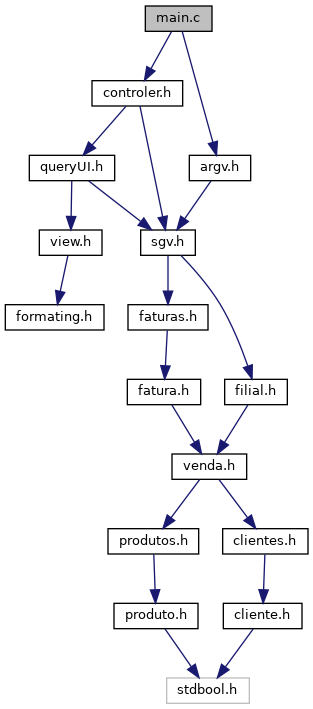
\includegraphics[width=0.4\textwidth]{dependency.png}\par
        \caption{Grafo de Dependências do projeto gerado pela ferramenta \textit{Doxygen}}
    \end{center}
\end{figure}

\chapter{Tabela de Tempos de Execução}

\begin{table}[H]
    \begin{center}
        \begin{tabular}{| c | c | c | c |}
            \hline
            & 1 Milhão & 3 Milhões & 5 Milhões \\
            \hline
            Load Time & 3.30 & 8.88 & 14.22 \\
            \hline
            Query 1.1 & 0.003 & 0.003 & 0.003 \\
            \hline
            Query 1.2 & 0.00001 & 0.00003 & 0.00001 \\
            \hline
            Query 1 & 0.004 & 0.003 & 0.004 \\
            \hline
            Query 2 & 0.003 & 0.003 & 0.003 \\
            \hline
            Query 3 & 0.0004 & 0.0003 & 0.0003 \\
            \hline
            Query 4 & 0.00007 & 0.0001 & 0.00008 \\
            \hline
            Query 5 & 0.000009 & 0.000008 & 0.000007 \\
            \hline
            Query 6 & 0.00002 & 0.00002 & 0.000007 \\
            \hline
            Query 7 & 0.0003 & 0.00005 & 0.00005 \\
            \hline
            Query 8 & 0.194 & 0.193 & 0.194 \\
            \hline
            Query 9 & 0.00003 & 0.00003 & 0.00003 \\
            \hline
            Query 10 & 0.00003 & 0.00003 & 0.00003 \\
            \hline

        \end{tabular}
        \caption{Tempo (em segundos) das queries para um dado número de vendas}
        \label{tab:benches}
    \end{center}
\end{table}

\end{document}
